\section{Modelos de Regresion}

Finalmente, vemos los modelos propuestos. Primero sin la libertad mundial como independiente, y luego con est\'a. Los resultados se muestran en la tablas \ref{regresiones} y \ref{regresiones1} de la p\'agina \pageref{regresiones} y \pageref{regresiones1}.

\begin{table}[H] \centering 
  \caption{Modelo de regresi\'on propuesto para los datos de departamentos de cabecera} 
  \label{regresiones} 
\begin{tabular}{@{\extracolsep{5pt}}lc} 
\\[-1.8ex]\hline 
\hline \\[-1.8ex] 
 & \multicolumn{1}{c}{\textit{Dependent variable:}} \\ 
\cline{2-2} 
\\[-1.8ex] & IDH \\ 
\hline \\[-1.8ex] 
 cabeLog & 0.013$^{***}$ \\ 
  & (0.004) \\ 
  & \\ 
 Constant & 0.634$^{***}$ \\ 
  & (0.055) \\ 
  & \\ 
\hline \\[-1.8ex] 
Observations & 32 \\ 
R$^{2}$ & 0.238 \\ 
Adjusted R$^{2}$ & 0.212 \\ 
Residual Std. Error & 0.037 (df = 30) \\ 
F Statistic & 9.347$^{***}$ (df = 1; 30) \\ 
\hline 
\hline \\[-1.8ex] 
\textit{Note:}  & \multicolumn{1}{r}{$^{*}$p$<$0.1; $^{**}$p$<$0.05; $^{***}$p$<$0.01} \\ 
\end{tabular} 
\end{table} 

Cras mattis, quam cursus pellentesque efficitur, metus nisi pharetra ipsum, blandit bibendum purus lacus nec enim. Vestibulum leo dui, ultrices et nibh a, accumsan finibus elit. Duis pellentesque ligula a justo volutpat dapibus. Donec in ligula eget ante aliquet convallis. Curabitur placerat nisi at justo euismod elementum. Fusce tristique risus pulvinar turpis interdum ultrices. Vivamus luctus congue dapibus. Nullam et commodo metus. Aenean tincidunt consequat mattis. Nunc ut lectus tempor, pretium nisi quis, pulvinar nisl. Interdum et malesuada fames ac ante ipsum primis in faucibus. Aliquam egestas feugiat turpis congue ullamcorper. Maecenas porta pulvinar erat a aliquet. Mauris scelerisque nibh quis bibendum dictum. Mauris at fringilla leo, vel dapibus ipsum. Pellentesque sit amet ex iaculis elit blandit lobortis.

Interdum et malesuada fames ac ante ipsum primis in faucibus. Proin mauris enim, interdum a tristique in, sagittis nec turpis. Sed in tristique felis, vitae tempus urna. Nulla facilisi. Ut pellentesque libero quis vulputate porta. Cras vitae risus est. In hac habitasse platea dictumst.

\begin{table}[H] \centering 
  \caption{Modelo de regresi\'on propuesto para los datos de todos los departamentos} 
  \label{regresiones1} 
\begin{tabular}{@{\extracolsep{5pt}}lc} 
\\[-1.8ex]\hline 
\hline \\[-1.8ex] 
 & \multicolumn{1}{c}{\textit{Dependent variable:}} \\ 
\cline{2-2} 
\\[-1.8ex] & IDH \\ 
\hline \\[-1.8ex] 
 cabeLog & 0.031$^{***}$ \\ 
  & (0.007) \\ 
  & \\ 
 restoLog & $-$0.030$^{***}$ \\ 
  & (0.010) \\ 
  & \\ 
 Constant & 0.766$^{***}$ \\ 
  & (0.065) \\ 
  & \\ 
\hline \\[-1.8ex] 
Observations & 32 \\ 
R$^{2}$ & 0.425 \\ 
Adjusted R$^{2}$ & 0.385 \\ 
Residual Std. Error & 0.033 (df = 29) \\ 
F Statistic & 10.706$^{***}$ (df = 2; 29) \\ 
\hline 
\hline \\[-1.8ex] 
\textit{Note:}  & \multicolumn{1}{r}{$^{*}$p$<$0.1; $^{**}$p$<$0.05; $^{***}$p$<$0.01} \\ 
\end{tabular} 
\end{table} 

\clearpage
\section{Exploraci\'on espacial}

Como acabamos de ver en la Tabla \ref{regresiones} en la p\'agina \pageref{regresiones}, si quisieras sintetizar la multidimensionalidad de nuestros indicadores, podr\'iamos usar tres de las cuatro variables que tenemos (un par de las originales tiene demasiada correlaci\'on). 

As\'i, propongo que calculemos conglomerados de departamentos usando toda la informaci\'on de tres de los indicadores. Como nuestras variables son ordinales utilizaremos un proceso de conglomeraci\'on usando la tecnica de k-means propuesta por \textbf{\cite{macqueen_methods_1966}}.El resultado de este proceso se muestra en la Figura \ref{mapa}. 

\begin{figure}[H]
\centering
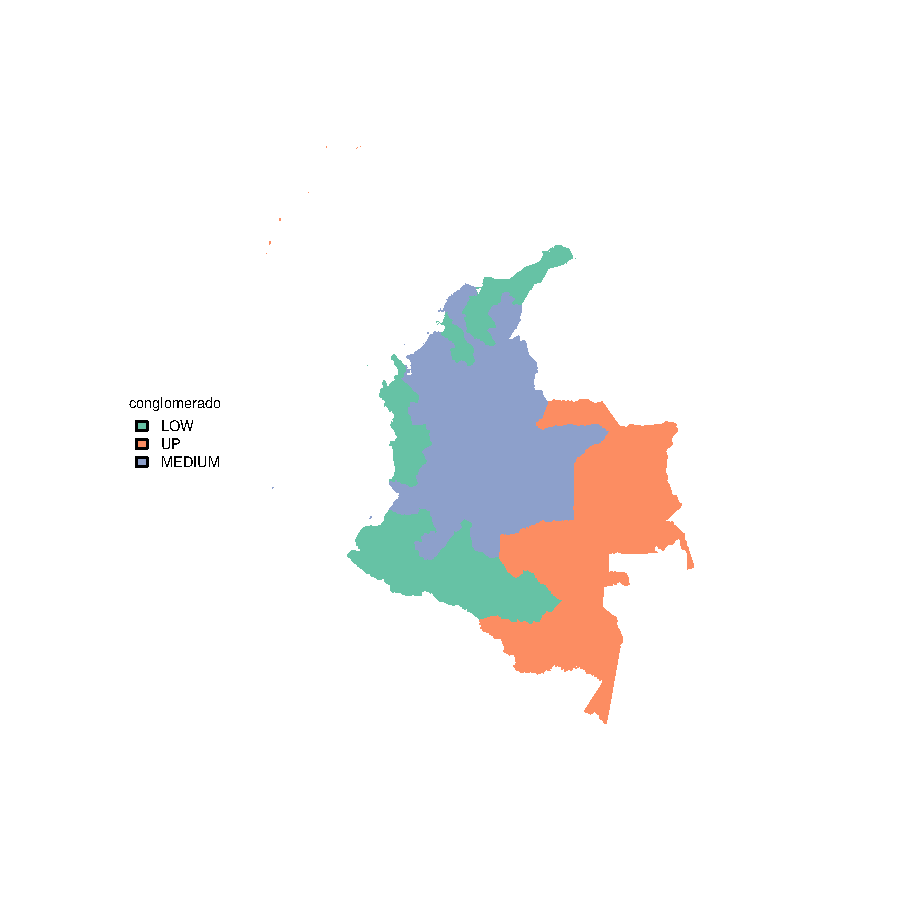
\includegraphics[width=\textwidth,trim={2cm 2cm 3cm 3cm},clip]{Modelos_regresion-plotMap1}
\caption{Histograma del IDH en Colombia para los 32 departamentos}
\label{mapa}
\end{figure}
\endinput
